A common case of the Nested class is an application that uses multiple parallel libraries at the same time, which could be developed 
using OpenMP, TBB, Cilkplus, C++11, and other parallel libraries. 
%In Figure~\ref{fig:cholesky}, 
For example, a Cholesky Factorization shown in Figure~\ref{fig:cholesky} uses OpenMP 
tasking and BLAS operations provided by Intel MKL library\footnote{The program was provided by Xavier Teruel from BSC demonstrating the interoperability problem for the INTERWinE project.}, 
which is a parallel math library. The runtime will then need to coordinate the two
parallel runtimes if the two do not integrate. %, e.g. each has its own instance during the program execution.
It is also posibble that multiple OpenMP runtime instances from either same or different libraries coexist, which
may incur even more challenges than the coexistence of different runtime instances, e.g. the naming conflict 
in the runtime. 
%These runtime instances could be created by user threads  OpenMP operations. 
\begin{figure}[h!]
  \centering
      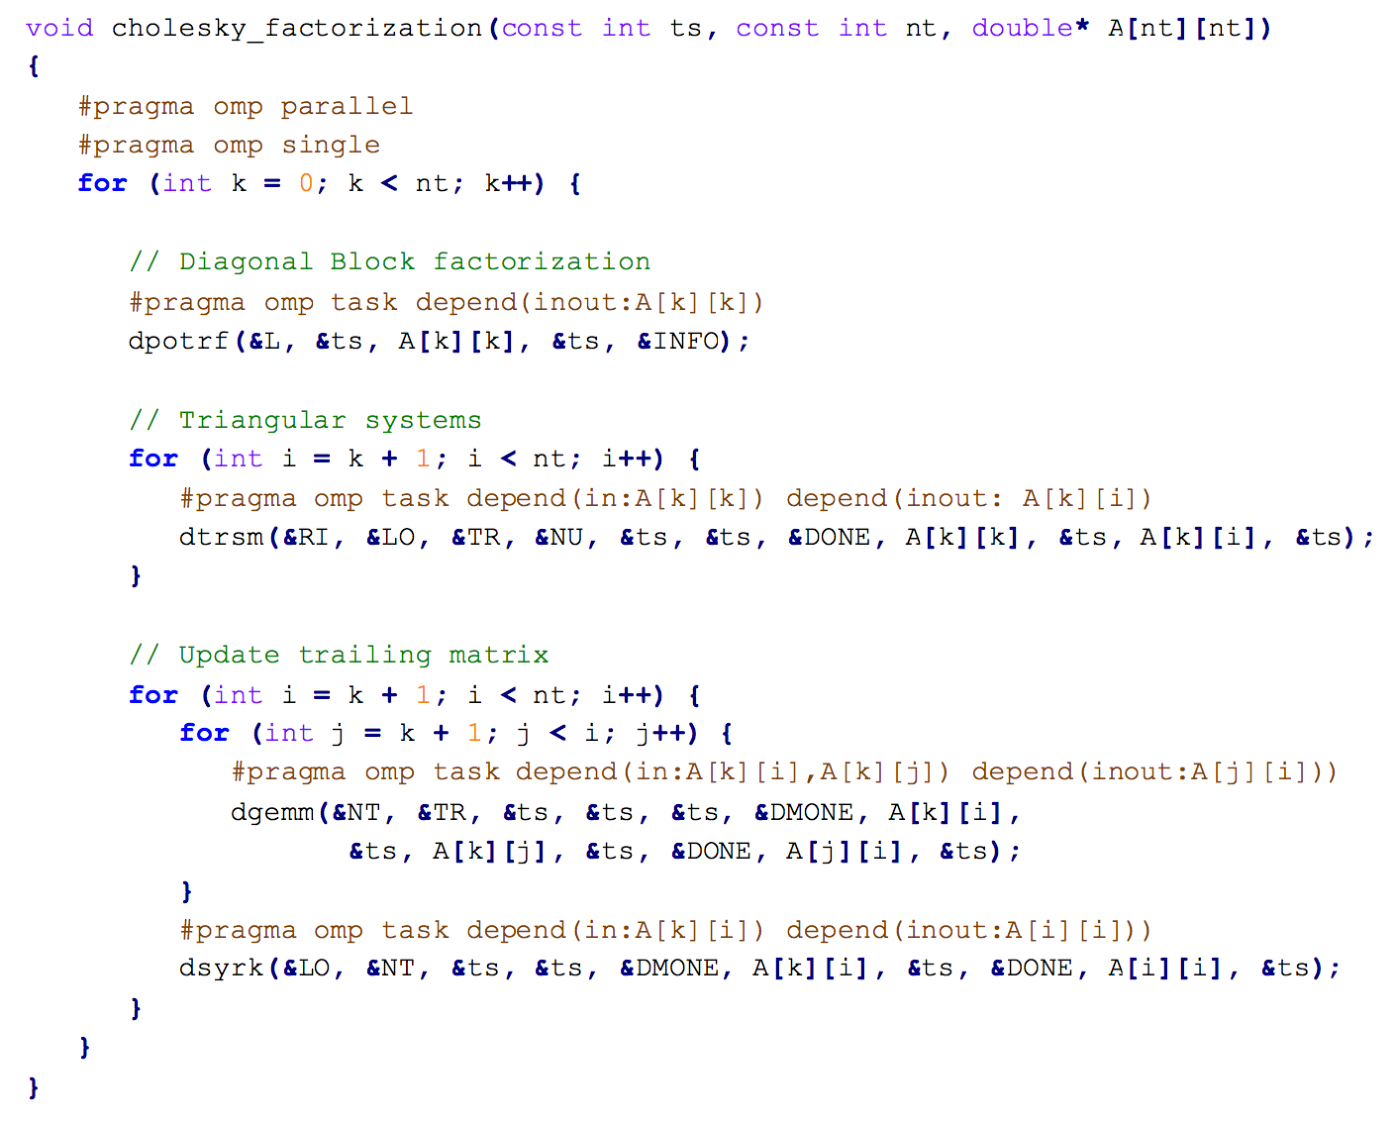
\includegraphics[width=0.75\textwidth]{images/cholesky}
      \caption{The Mixed Use of OpenMP Tasking and Intel MKL Library for Cholesky Factorization~\cite{intertwine}}
 \label{fig:cholesky}
\end{figure}
